\documentclass[
  a4paper,uplatex,dvipdfmx,10pt,
  xcolor = {dvipsnames,svgnames},
  hyperref ={colorlinks=true,citecolor=Navy,linkcolor=NavyBlue,urlcolor=purple}
]{beamer}
\renewcommand{\baselinestretch}{1.2}

% ---refer `texdoc xcolor' at the command line---

% ---Display \subsubsection at the Index
% \setcounter{tocdepth}{3}

% ---Setting about the geometry of the document----
% \usepackage{a4wide}
% \pagestyle{empty}

% ---Physics and Math Packages---
\usepackage{amssymb,amsfonts,amsthm,mathtools}
\usepackage{physics,braket,bm}

% ---underline---
\usepackage{ulem}

% ---cancel---
\usepackage{cancel}

% --- surround the texts or equations
% \usepackage{fancybox,ascmac}

% ---settings of theorem environment---
% \usepackage{amsthm}
% \theoremstyle{definition}

% ---settings of proof environment---
% \renewcommand{\proofname}{\textbf{証明}}
% \renewcommand{\qedsymbol}{$\blacksquare$}

% ---Ignore the Warnings---
\usepackage{silence}
\WarningFilter{latexfont}{Some font shapes,Font shape}
\ExplSyntaxOn
\msg_redirect_name:nnn{hooks}{generic-deprecated}{none}
\ExplSyntaxOff

% ---Insert the figure (If insert the `draft' at the option, the process becomes faster.)---
\usepackage{graphicx}
% \usepackage{subcaption}

% ----Add a link to a text---
\usepackage{url,hyperref}
\usepackage{xcolor}
\usepackage{pxjahyper}

% ---Tikz---
\usepackage{tikz,pgf,pgfplots,circuitikz}
\pgfplotsset{compat=1.15}
\usetikzlibrary{intersections,arrows.meta,angles,calc,3d,decorations.pathmorphing,positioning}

% ---Add the section number to the equation, figure, and table number---
\makeatletter
   \renewcommand{\theequation}{\thesection.\arabic{equation}}
   \@addtoreset{equation}{section}
   
   \renewcommand{\thefigure}{\thesection.\arabic{figure}}
   \@addtoreset{figure}{section}
   
   \renewcommand{\thetable}{\thesection.\arabic{table}}
   \@addtoreset{table}{section}
\makeatother

% ---enumerate---
% \renewcommand{\labelenumi}{$\arabic{enumi}.$}
% \renewcommand{\labelenumii}{$(\arabic{enumii})$}

% ---beamer settings---
\usefonttheme{professionalfonts}
% \usefonttheme{serif}
\usecolortheme{seahorse}
\setbeamercolor{structure}{fg=Turquoise}
\setbeamercolor{local structure}{fg=Turquoise}
\setbeamertemplate{itemize item}[ball]
\setbeamertemplate{enumerate item}[circle]
\setbeamercolor{bibliography entry author}{fg=black}
\setbeamercolor{bibliography item}{fg=black}
\setbeamertemplate{frametitle continuation}{}
\setbeamertemplate{footline}[frame number]
\setbeamertemplate{navigation symbols}{} 

% ---Fonts---
\renewcommand{\familydefault}{\sfdefault}
\renewcommand{\kanjifamilydefault}{\gtdefault}
% \usepackage{newtxmath}
\mathversion{bold}

% ---
\usepackage{usebib}
\newbibfield{author} 
\newbibfield{year} 
\newbibfield{journal} 
\newbibfield{doi} 
\bibinput{hoge}

\makeatletter
\newcommand*{\journal}{\begingroup\@makeother\#\@mylink}
\newcommand*{\@mylink}[1]{\href{http://dx.doi.org/\usebibentry{#1}{doi}}{\usebibentry{#1}{journal}}\endgroup} 
\makeatother

\newcommand*{\citefone}[2]{
  \begin{tikzpicture}[remember picture, overlay]
    \node[anchor=north east, align=left] at ($(current page.north east)-(0,1.05)$){
    {\tiny
      \cite{#1}
      #2,
      \journal{#1}
      (\usebibentry{#1}{year}).
    }
    };
  \end{tikzpicture}
}
\newcommand*{\citeftwo}[4]{
  \begin{tikzpicture}[remember picture, overlay]
    \node[anchor=north east, align=left] at ($(current page.north east)-(0,1.05)$){
    {\tiny
      \cite{#1}
      #2,
      \journal{#1}
      (\usebibentry{#1}{year}).
    }
    \\[-1.8ex]
    {\tiny
      \cite{#3}
      #4,
      \journal{#3}
      (\usebibentry{#3}{year}).
    }
    };
  \end{tikzpicture}
}
\newcommand*{\citefthree}[6]{
  \begin{tikzpicture}[remember picture, overlay]
    \node[anchor=north east, align=left] at ($(current page.north east)-(0,1.05)$){
    {\tiny
      \cite{#1}
      #2,
      \journal{#1}
      (\usebibentry{#1}{year}).
    }
    \\[-1.8ex]
    {\tiny
      \cite{#3}
      #4,
      \journal{#3}
      (\usebibentry{#3}{year}).
    }
    \\[-1.8ex]
    {\tiny
      \cite{#5}
      #6,
      \journal{#5}
      (\usebibentry{#5}{year}).
    }
    };
  \end{tikzpicture}
}


% ---Title---
\title{
  卒論\ 中間発表
  \\
  {\Large Moduli stabilization for magnetized D-brane models (??)}
  \\
  v2
}
\author{宮根 一樹}
\date{2023年12月14日}

\begin{document}

\begin{frame}
  \titlepage
  \begin{center}
    \textcolor{DarkMagenta}{
      先日はあんな発表のためにご辛抱ありがとうございました.
      \\
      修正や加筆はこの色で行いました.
    }
  \end{center}
\end{frame}

\setbeamertemplate{section in toc}[circle]
\setbeamertemplate{subsection in toc}[ball]
\begin{frame}[allowframebreaks]
  \frametitle{目次}
  \tableofcontents
\end{frame}


\section{イントロダクション}

\begin{frame}
  \frametitle{\thesection\ \secname}
  \color{DarkMagenta}

  素粒子標準模型
  \begin{itemize}
    \color{DarkMagenta}
    \item 
    実験でよく結果が確認されている
    \item 
    $SU(3)_{C}\times SU(2)_{L}\times U(1)_{Y}$のゲージ理論
    \item 
    左右が非対称な理論
  \end{itemize}

  \vspace{10pt}

  標準模型の問題点
  \begin{itemize}
    \color{DarkMagenta}
    \item 
    重力が含まれていない
    \item 
    世代やフレーバーの違いで大きく質量が変わる
  \end{itemize}
  {\hspace{8cm} など}

\end{frame}

\begin{frame}
  \frametitle{\thesection\ \secname}
  \color{DarkMagenta}

  超弦理論
  \begin{itemize}
    \color{DarkMagenta}
    \item 
    重力を含む
    \item 
    10次元で無矛盾な理論
  \end{itemize}

  \vspace{10pt}

  現実的なモデルを得るためには
  \begin{itemize}
    \color{DarkMagenta}
    \item 
    \uwave{余剰次元を観測できないほどにコンパクト化}
    \item 
    カイラリティやゲージ群を再現
    \item 
    世代やフレーバ,そして質量を再現
  \end{itemize}

  \pause 

  \begin{tikzpicture}[remember picture, overlay]
    \node[anchor=north east, align=left] at ($(current page.north east)-(0,5)$){
      {
        \small
        今回の研究の関心
      }
    };
    \draw[->](9.0,2.2)--(7.7,2.0);
  \end{tikzpicture}

\end{frame}

% \begin{frame}
%   \frametitle{\thesection\ \secname}
%   \color{DarkMagenta}

%   モジュライ固定


%   \pause

%   \vspace{1cm}

%   {\large
%   \vspace{10pt}
%   \begin{equation}
%     \text{超弦理論}
%     \xleftrightarrow{\text{\ 余剰次元の大きさ\ }}
%     \underbrace{
%     \text{モジュライ}    
%     \xleftrightarrow{\text{\ VEVの決定\ }}
%     \text{有効理論}
%     }_{\text{今回の研究}}
%     \nonumber
%   \end{equation}
%   }

% \end{frame}


\section{レビュー}

\begin{frame}
  \frametitle{\thesection.\ \secname}

  \begin{tikzpicture}[scale=1.0, grow'=up]
    \tikzset{block/.style={rectangle, fill=cyan!10, text width=2.5cm, text centered, rounded corners, minimum height=1.5cm}};
    \node[block] {モジュライ固定} [level distance=3cm, sibling distance=4cm, edge from parent/.style={<-,draw}]
        child{ node[block] {モジュライ} 
          child{ node[block] {コンパクト化} }
        }
        child{ node[block] {SUSY} }
        child{ node[block] {磁場} };
 \end{tikzpicture}  
  
\end{frame}


\subsection{コンパクト化}

\begin{frame}
  \frametitle{\thesection.\thesubsection\ \subsecname}  

  \citeftwo{Arkani-Hamed_HigherDimensional_2002}{N. Arkani-Hamed, T. Gregoire, and J. Wacker}{Abe_SuperfieldDescription_2012}{H. Abe, T. Kobayashi, H. Ohki, and K. Sumita}

  10次元($M,N$) $\rightarrow$ 4次元ミンコフスキー $+$ 余剰次元.
  \begin{itemize}
    \item 
    例えば,座標は$X^{M}=(x^{\mu},y^{m})$
  \end{itemize}

  \vspace{-10pt}

  \begin{center}
    $\downarrow$

    トーラス方向だけの座標を取り直す
  \end{center}

  \vspace{10pt}

  例えば
  \begin{equation}
    \left\{
      \begin{alignedat}{1}
        z^{1}
        &\equiv
        \frac{1}{2}(y^4+\tau_{1}y^5)
        \nonumber
        \\
        \tilde{A}_{1}
        &\equiv
        -
        \frac{1}{\Im\tau_{1}}(\tau_{1}^{*}A_{4}-A_{5})
      \end{alignedat}
    \right.
  \end{equation}
  \color{DarkMagenta}
  
  \begin{itemize}
    \color{DarkMagenta}
    \item 
    $\tau_{i}$は複素数
    \item 
    $
    (y_{4},y_{5})
    \rightarrow
    (z_{1},\bar{z}_{1})
    ,\ 
    (y_{6},y_{7})
    \rightarrow
    (z_{2},\bar{z}_{2})
    ,\ 
    (y_{8},y_{9})
    \rightarrow
    (z_{3},\bar{z}_{3})
    $
  \end{itemize}

  以後は$\tilde{A}_{i}$を$A_{i}$と書く.

\end{frame}

\begin{frame}
  \frametitle{\thesection.\thesubsection\ \subsecname}  

  \citeftwo{Arkani-Hamed_HigherDimensional_2002}{N. Arkani-Hamed, T. Gregoire, and J. Wacker}{Abe_SuperfieldDescription_2012}{H. Abe, T. Kobayashi, H. Ohki, and K. Sumita}

  境界条件を
  \begin{equation}
    y^{m}\sim y^{m}+2
    \longrightarrow
    z^{i}\sim z^{i}+1
    \ \text{\&}\ 
    z^{i}\sim z^{i}+\tau^{i}
    .
    \nonumber
  \end{equation}
  と入れる.\color{DarkMagenta}これで$z_{1},z_{2},z_{3}$はトーラスの座標になる.

  \vspace{1cm}

  \begin{center}
    \mbox{
      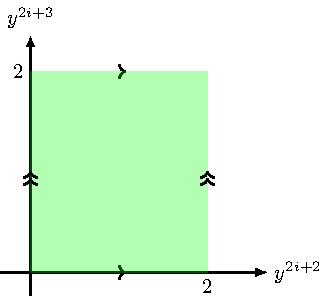
\includegraphics[keepaspectratio,width=0.38\linewidth]{fig/torus/torus1.pdf}
    }
    \mbox{
      \raisebox{1.5cm}{
        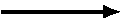
\includegraphics[keepaspectratio,width=0.10\linewidth]{fig/arrow/arrow.pdf} 
      }
    }   
    \mbox{
      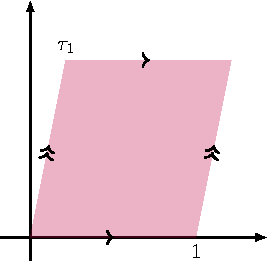
\includegraphics[keepaspectratio,width=0.38\linewidth]{fig/torus/torus2.pdf}   
    } 
  \end{center}
  
\end{frame}

\begin{frame}
  \frametitle{\thesection.\thesubsection\ \subsecname}  

  \citeftwo{Arkani-Hamed_HigherDimensional_2002}{N. Arkani-Hamed, T. Gregoire, and J. Wacker}{Abe_SuperfieldDescription_2012}{H. Abe, T. Kobayashi, H. Ohki, and K. Sumita}

  \textcolor{DarkMagenta}{境界条件に対する計量}
  \begin{gather}
    g^{(i)}
    =
    (2\pi R_{i})^2
    \begin{pmatrix}
      1 & \Re\tau_{i} \\
      \Re\tau_{i} & |\tau_{i}|^2
    \end{pmatrix}
    \text{:トーラスの計量}
    \nonumber
    \\
    \mathcal{A}^{(i)}
    =
    (2\pi R_{i})^2
    \Im\tau_{i}
    \text{:トーラスの面積}
    \label{area_tau}
  \end{gather}

  \vspace{10pt}

  \color{black}

  トーラスの座標$z^{i}$での計量
  \begin{gather}
    \dd s^{2}_{6}
    =
    2h_{i\bar{j}}\dd z^{i}\dd \bar{z}^{\bar{j}}
    ,
    \nonumber
    \\
    h_{i\bar{j}}
    =
    2(2\pi R_{i})^2 \delta_{i\bar{j}}
    .
    \nonumber
  \end{gather}

\end{frame}


\subsection{超対称性}

\begin{frame}
  \frametitle{\thesection.\thesubsection\ \subsecname}  
  \begin{tikzpicture}[remember picture, overlay]
    \node[anchor=north east, align=left] at ($(current page.north east)-(0,1.05)$){
    {\tiny
      \cite{Wess_SupersymmetrySupergravity_1992}
      J. Wess and J. Bagger, \textit{Supersymmetry and Supergravity.}
    }
    };
  \end{tikzpicture}
  \color{DarkMagenta}

  超弦理論の低エネルギー有効理論
  \begin{itemize}
    \color{DarkMagenta}
    \item 
    10次元超対称ヤン・ミルズ理論
    \item 
    超重力理論
  \end{itemize}
  など

  \vspace{10pt}

  超対称性
  \begin{itemize}
    \color{DarkMagenta}
    \item 
    ボゾンとフェルミオンの変換
    \item 
    次のような利点(\href{https://www-hep.phys.se.tmu.ac.jp/FPWS2014/uploads/7-2014.12.8_Flavour_Jinnouchi.pdf}{があるそうです})
    \begin{itemize}
      \color{DarkMagenta}
      \item 
      発散が相殺されるケースがある
      \item 
      ダークマターの候補があるとか
    \end{itemize}
  \end{itemize}

\end{frame}


\begin{frame}
  \frametitle{\thesection.\thesubsection\ \subsecname}  
  \begin{tikzpicture}[remember picture, overlay]
    \node[anchor=north east, align=left] at ($(current page.north east)-(0,1.05)$){
    {\tiny
      \cite{Wess_SupersymmetrySupergravity_1992}
      J. Wess and J. Bagger, \textit{Supersymmetry and Supergravity.}
    }
    };
  \end{tikzpicture}
  \color{DarkMagenta}

  超対称多重項で実現
  \begin{equation}
    V
    =
    \{
      A_{\mu}
      ,
      \lambda_{0}
      ,
      \bar{\lambda}_{0}
      ,
      D
    \}
    ,\quad
    \phi_{i}
    =
    \{
      A_{i},\lambda_{i},F_{i}
    \}
    \nonumber
  \end{equation}

  \begin{center}
    \begin{itemize}
      \color{DarkMagenta}
      \item 
      $i=1,2,3$はトーラスの添え字
      \item 
      $A_{\mu},\lambda_{0},\cdots$などが次元が4のときの場
      \item 
      $D,F_{i}$は補助場
    \end{itemize}
  \end{center}

  \vspace{10pt}

  SUSY対称なポテンシャル
  \begin{itemize}
    \color{DarkMagenta}
    \item 
    スーパーポテンシャル$W$
    ,
    ケーラーポテンシャル$K$
    \item 
    SUSY不変性を見るときに重要
  \end{itemize}

\end{frame}


\subsection{磁場の導入}
\label{magnetic_flux}

\begin{frame}
  \frametitle{\thesection.\thesubsection\ \subsecname}

  \citefone{Abe_SuperfieldDescription_2012}{H. Abe, T. Kobayashi, H. Ohki, and K. Sumita}

  \color{DarkMagenta}

  \begin{itemize}
    \color{DarkMagenta}
    \item 
    今回考える10次元超対称ヤン・ミルズ理論では
    \begin{equation}
      D
      =
      -h^{\bar{i}j}
      \left(  
        \bar{\partial}_{\bar{i}}A_{j}
        +
        \partial_{j}\bar{A}_{\bar{i}}
        +
        \frac{1}{2}[\bar{A}_{\bar{i}},A_{j}]
      \right)
      \nonumber
    \end{equation}

    \item 
    SUSYを保つ$D$の真空期待値の条件
    \begin{equation}
      \ev*{D}
      =
      -h^{\bar{i}j}
      \left(  
        \bar{\partial}_{\bar{i}}\ev*{A_{j}}
        +
        \partial_{j}\ev*{\bar{A}_{\bar{i}}}
        +
        \frac{1}{2}[\ev*{\bar{A}_{\bar{i}}},\ev*{A_{j}}]
      \right)
      =
      0
      \label{SUSY_cond_D}
    \end{equation}
  \end{itemize}

\end{frame}

\begin{frame}
  \frametitle{\thesection.\thesubsection\ \subsecname}

  \citefone{Abe_SuperfieldDescription_2012}{H. Abe, T. Kobayashi, H. Ohki, and K. Sumita}

  真空期待値を\textcolor{DarkMagenta}{次のように決める}.
  \begin{equation}
    \ev*{A_{i}}
    =
    \frac{\pi}{\Im \tau_{i}}\textcolor{Navy}{M^{(i)}}\bar{z}_{i}
    ,
    \nonumber
  \end{equation}
  \begin{equation}
    \textcolor{Navy}{
      M^{(i)}
    }
    \textcolor{Navy}{
      =
      \begin{pmatrix}
        M_{1}^{(i)} &0 &\cdots & 0\\
        0&M_{2}^{(i)}&\cdots&0\\
        \vdots& \vdots& \ddots &\vdots \\
        0 & 0 & \cdots & M_{N}^{(i)}
      \end{pmatrix}
    }
    .
  \end{equation}

  \begin{itemize}
    \color{DarkMagenta}
    \item 
    $M_{a}^{(i)}$は整数
    \item 
    $M^{(i)}$はトーラス上の磁場
    $\rightarrow$
    $F_{45}=\pi M^{(1)}$など
    \item 
    ブロック対角化でより小さいゲージ対称性
    $$
      U(N)
      \rightarrow
      U(N_1)
      \times
      U(N_2)
      \times
      \cdots
      \times
      U(\tilde{N})
    $$
  \end{itemize}

\end{frame}


\begin{frame}
  \frametitle{\thesection.\thesubsection\ \subsecname}

  \citeftwo{Abe_SuperfieldDescription_2012}{H. Abe, T. Kobayashi, H. Ohki, and K. Sumita}{Abe_AhlerModuli_2017}{H. Abe, T. Kobayashi, K. Sumita, and S. Uemura}

\begin{itemize}
  \item
  補助場$D^{a}$が作るスカラーポテンシャル
  \begin{align}
    V^{(D)}
    &=
    \frac{1}{2}(D^{a})^2
    ,
    \label{scalar_PE_D}
    \\
    D_{a}
    &=
    \sum_{r}
    \frac{\pi M_{a}^{(r)}}{\mathcal{A}^{(r)}}
    .
    \label{D}
  \end{align}

  \color{DarkMagenta}

  真空期待値を表すブラケット$\ev*{\ }$は省略

  \item 

  \hyperlink{SUSY_cond_D}{SUSYを保つための条件}
  \begin{equation} 
    D_{a}
    =   
    \sum_{r}
    \frac{\pi M_{a}^{(r)}}{\mathcal{A}^{(r)}}
    =
    0
    \quad
    (a=1,2,3)
  \end{equation}

\end{itemize}

\end{frame}

\subsection{モジュライ固定と\texorpdfstring{$F$}{F}-term uplifting}

\begin{frame}
  \frametitle{\thesection.\thesubsection\ \subsecname}
  \color{DarkMagenta}

  モジュライ$T_{r}$
  \begin{itemize}
    \color{DarkMagenta}
    \item 
    定義
    \begin{equation}
      \Re T_{r}
      \equiv
      e^{-\ev*{\phi_{10}}}
      \mathcal{A}^{(r)}
      \nonumber
    \end{equation}
    $\mathcal{A}^{(r)}$は$r$番目のトーラスの面積
    ,
    $\phi_{10}$はディラトン
    \begin{itemize}
      \color{DarkMagenta}
      \item 
      高エネルギーの理論では(ダイナミカルな)スカラー場
      \item 
      10次元のヤン・ミルズ理論の結合定数との関係は$g=e^{-\ev*{\phi_{10}}}$
    \end{itemize}
    \item 
    このモジュライの真空期待値を決定すべき
  \end{itemize}

\end{frame}


\begin{frame}
  \frametitle{\thesection.\thesubsection\ \subsecname}

  \citefthree{Kachru_SitterVacua_2003}{S. Kachru, R. Kallosh, A. Linde, and S. P. Trivedi}{Abe_ModuliStabilization_2007a}{H. Abe, T. Higaki, T. Kobayashi, and Y. Omura}{Abe_MoreFterm_2007a}{H. Abe, T. Higaki, and T. Kobayashi}

  \uline{KKLTモデル}\cite{Kachru_SitterVacua_2003}

  \vspace{10pt}

  ポテンシャル
  \begin{equation}
    K
    =
    -n_{T}\log(T+\bar{T})
    ,\ 
    W
    =
    c-Ae^{-aT}
    .
    \label{PE_KKLT}
  \end{equation}

  スカラーポテンシャル
  \begin{gather}
    V
    =
    e^{K}(K^{T\bar{T}}|D_{T}W|^2-3|W|^2)
    \nonumber
    \\
    D_{T}W
    =
    -e^{-K/2}K_{T\bar{T}}F^{\bar{T}}
    \propto
    F^{\bar{T}}
    \nonumber
  \end{gather}
  \vspace{-10pt}
  \begin{itemize}
    \item 
    $D_{T}W=0$では,SUSYが保たれている
    \item 
    $D_{T}W=0$かつ$a\Re T\sim\log A/c$のときにモジュライ$T$は安定
  \end{itemize}
  \pause

  \color{DarkRed}

  \begin{center}
    $T$が安定のところでは$V=-3e^{K}|W|^2<0$
    
    \vspace{5pt}

    $V=0$のほうが嬉しいらしいので,$\partial_{T}V=0$で$V=0$を目指す
  \end{center}

  \color{black}

\end{frame}


\begin{frame}
  \frametitle{\thesection.\thesubsection\ \subsecname}

  \citeftwo{Abe_ModuliStabilization_2007a}{H. Abe, T. Higaki, T. Kobayashi, and Y. Omura}{Abe_MoreFterm_2007a}{H. Abe, T. Higaki, and T. Kobayashi}

  \hyperlink{PE_KKLT}{KKLTモデルのポテンシャル}を変える(Polonyi-KKLTモデル)
  \begin{equation}
    K
    =
    \textcolor{ForestGreen}{|\Phi|^2}
    -
    n_{T}\log(T+\bar{T})
    ,\ 
    W
    =
    c
    +
    \textcolor{DarkRed}{\mu^2\Phi}
    -
    Ae^{-aT}
    \label{PE_Polonyi_KKLT}
  \end{equation}

  \vspace{10pt}

  パラメターの仮定
  \begin{equation}
    A\sim 1
    ,\ 
    a\gg 1
    ,\ 
    c,\mu^{2}\ll 1
    \nonumber
  \end{equation}

\end{frame}

\begin{frame}
  \frametitle{\thesection.\thesubsection\ \subsecname}

  \citeftwo{Abe_ModuliStabilization_2007a}{H. Abe, T. Higaki, T. Kobayashi, and Y. Omura}{Abe_MoreFterm_2007a}{H. Abe, T. Higaki, and T. Kobayashi}

  analyticにやりたいので
  \begin{itemize}
    \item 
    極小の点にあたりをつける
    $\longrightarrow$
    基準点
    \item 
    その点がlocal minimumであることを正当化
  \end{itemize}

  \pause

  \vspace{10pt}

  基準点$(\phi,t)$は
  \begin{gather}
    \left.
      V_{\Phi}
    \right|_{0}
    =
    0
    ,\ 
    \left.
      D_{T}W
    \right|_{0}
    =
    0
    ,
    \label{ref_point_pol}
    \\
    \left.
      D_{\Phi}W
    \right|_{0}
    \neq
    0
    \nonumber    
  \end{gather}
  を満たす点

  記号の意味は
  \begin{equation}
    \left.
      f(\Phi,T)
    \right|_{0}
    \equiv
    f(\phi,t)
    .
    \nonumber
  \end{equation}

\end{frame}

\begin{frame}
  \frametitle{\thesection.\thesubsection\ \subsecname}

  \citeftwo{Abe_ModuliStabilization_2007a}{H. Abe, T. Higaki, T. Kobayashi, and Y. Omura}{Abe_MoreFterm_2007a}{H. Abe, T. Higaki, and T. Kobayashi}

  \begin{itemize}
    \item 

    \hyperlink{ref_point_pol}{基準点}の条件と$
    \left.
      V
    \right|_{0}
    =
    0$より$(\phi,t)$は
    \begin{equation}
      \phi
      =
      \sqrt{3}-1
      ,\ 
      \mu^{-2}(c-Ae^{-at})
      =
      2-\sqrt{3}
      \nonumber
    \end{equation}

    \item 
    2つめから$t=\mathcal{O}(1)$ほど
    $\rightarrow$
    $K\left.\right|_{0}$も$\mathcal{O}(1)$

    \item 
    $\delta\Phi,\delta T$:基準点$(\phi,t)$と\textcolor{DarkMagenta}{実際の最小値$(\Phi,T)$との差}
    \begin{equation}
      \Phi
      =
      \phi
      +
      \delta\Phi
      ,\ 
      T
      =
      t
      +
      \delta T
      .
      \nonumber
    \end{equation}
  
    \item 
    $\delta \Phi/\phi,\ \delta T/t\ll 1$であることを確認
  \end{itemize}

\end{frame}

\begin{frame}
  \frametitle{\thesection.\thesubsection\ \subsecname}

  \citeftwo{Abe_ModuliStabilization_2007a}{H. Abe, T. Higaki, T. Kobayashi, and Y. Omura}{Abe_MoreFterm_2007a}{H. Abe, T. Higaki, and T. Kobayashi}

  \textcolor{DarkMagenta}{ちゃんと2次までやるべき}
  \color{gray}

  $W$と$D_{T}W$を展開
  \begin{align}
    W
    &=
    W
    \left.\right|_{0}
    +
    W_{T}
    \left.\right|_{0}
    \delta T
    +
    W_{\Phi}
    \left.\right|_{0}
    \delta \Phi
    +\cdots
    \nonumber
    \\
    &\sim
    \mu^2
    +
    Aae^{-at}\delta T
    +
    \mu^2
    \delta\Phi
    ,
    \nonumber
    \\
    D_{T}W
    &=
    D_{T}W
    \left.\right|_{0}    
    +
    (D_{T}W)_{T}
    \left.\right|_{0}    
    \delta T
    +
    (D_{T}W)_{\Phi}
    \left.\right|_{0}    
    \delta \Phi
    +
    \cdots
    \nonumber
    \\
    &\sim
    -Aa^{2}e^{-at}
    \delta T
    -
    \uwave{
      \frac{\mu^2n_{T}}{2t}\delta\Phi
    }
    \nonumber
    \\
    &\hspace{3.2cm}
    +
    \left(  
      \frac{\mu^2n_{T}}{4t^2}
      \delta T
      -
      \frac{Aan_{T}}{2t}e^{-at}
      \delta T
    \right)
    \nonumber
  \end{align}
  
  カッコでくくったのは,今後無視していくつもりのterm.

\end{frame}

\begin{frame}
  \frametitle{\thesection.\thesubsection\ \subsecname}

  \citeftwo{Abe_ModuliStabilization_2007a}{H. Abe, T. Higaki, T. Kobayashi, and Y. Omura}{Abe_MoreFterm_2007a}{H. Abe, T. Higaki, and T. Kobayashi}

  \color{gray}

  $D_{\Phi}W$と$F^{T}$もestimateできて
  \begin{align}
    D_{\Phi}W
    &=
    \mu^2
    +
    (\sqrt{3}-1)
    \left(  
      \mu^2
      +
      Aae^{-at}\delta T
      +
      \mu^2
      \delta\Phi     
      +
      \cdots 
    \right)
    \nonumber
    \\
    &\sim
    \sqrt{3}\mu^2
    +
    Aae^{-at}
    \delta T
    +
    \mu^2
    \delta\Phi 
    ,     
    \nonumber
    \\
    F^{T}
    &\sim
    e^{K\left.\right|_{0}/2}
    \frac{2t}{n_{T}}
    \left(        
      a^2Ae^{-at}
      \delta T
      +
      \frac{\mu^2n_{T}}{2t}\delta\Phi
    \right)
    .
    \nonumber
  \end{align}

  スカラーポテンシャルは
  \begin{align}
    V
    &=
    e^{K}((D_{\Phi}W)(D_{\bar{\Phi}}\bar{\Phi})-3W\bar{W})
    +
    K_{T\bar{T}}F^{T}\bar{F}^{\bar{T}}
    \nonumber
    \\
    &\sim
    e^{K\left.\right|_{0}}
    \left\{  
      (D_{\bar{\Phi}}\bar{W})\left.\right|_{0}
      (D_{\Phi}W)
      -
      3\bar{W}\left.\right|_{0}W
    \right\}
    +
    K_{T\bar{T}}\bar{F}^{\bar{T}}\left.\right|_{0}F^{T}
    \nonumber
  \end{align}
  として計算する.本当は$\bar{W}W\left.\right|_{0}=\bar{W}\left.\right|_{0}W+\bar{W}W\left.\right|_{0}$と対称的に組むべきだが,VEVをとったら実になって2(つまり$\mathcal{O}(1)$)になるため

\end{frame}

\begin{frame}
  \frametitle{\thesection.\thesubsection\ \subsecname}

  \citeftwo{Abe_ModuliStabilization_2007a}{H. Abe, T. Higaki, T. Kobayashi, and Y. Omura}{Abe_MoreFterm_2007a}{H. Abe, T. Higaki, and T. Kobayashi}

  \color{gray}

  先ほどの$V$に$\delta T,\delta \Phi$の1次までの展開をいれると
  \begin{align}
    V
    &\sim
    e^{K\left.\right|_{0}}
    \left\{  
      \sqrt{3}\mu^2
      \cdot
      (\sqrt{3}\mu^2
      +
      Aae^{-at}
      \delta T
      +
      \mu^2
      \delta\Phi )
    \right.
    \nonumber
    \\
    &\hspace{3cm}
    -
    3\mu^2
    \cdot    
    (\mu^2
    +
    Aae^{-at}\delta T
    +
    \mu^2
    \delta\Phi  )
    \left.\right\}
    \nonumber
    \\
    &\hspace{1cm}
    +
    K_{T\bar{T}}
    e^{K\left.\right|_{0}/2}
    \frac{2t}{n_{T}}
    \left(  
      a^2Ae^{-at}
      \delta T
      +
      \frac{\mu^2n_{T}}{2t}\delta\Phi
    \right)
    \cdot
    F^{T}
    .
    \nonumber
    \\
    &\sim
    e^{K\left.\right|_{0}}
    \left[  
      \left(  
        ae^{-K\left.\right|_{0}/2}F^{T}
        -
        \sqrt{3}\mu^2
      \right)
      aAe^{-at}
      \delta T
    \right.
    \nonumber
    \\
    &\hspace{2cm}
    \left.
      +
      \mu^2
      \left\{
        \frac{n_{t}}{2t}
        e^{-K\left.\right|_{0}/2}  
        F^{T}
        -
        (3-\sqrt{3})
        \mu^2
      \right\}
      \delta\Phi
    \right]
    .
    \nonumber
  \end{align}

\end{frame}

\begin{frame}
  \frametitle{\thesection.\thesubsection\ \subsecname}

  \citeftwo{Abe_ModuliStabilization_2007a}{H. Abe, T. Higaki, T. Kobayashi, and Y. Omura}{Abe_MoreFterm_2007a}{H. Abe, T. Higaki, and T. Kobayashi}

  \color{gray}

  したがって,停留条件$V_{\delta T}=0\ \&\ V_{\delta \Phi}=0$から
  \begin{align}
    &
    V_{\delta T}
    =
    0
    \quad
    \longrightarrow
    \quad
    F^{T}
    =
    \sqrt{3}
    \mu^2 a^{-1}e^{K/2}
    \sim
    \frac{\mu^2}{a}
    \ll 
    1
    ,
    \label{variationofT_F}
    \\
    &
    V_{\delta \Phi}
    =
    0
    \quad
    \longrightarrow
    \quad
    F^{T}
    =
    (3
    -
    \sqrt{3})
    \mu^2\frac{2t}{n_{T}} a^{-1}e^{K/2}
    \sim
    \mu^2
    \ll 
    1
    .
    \label{variationofPhi_F}
  \end{align}

  ただし,$\cdot\left.\right|_{0}$の記号は省略している.

\end{frame}

\begin{frame}
  \frametitle{\thesection.\thesubsection\ \subsecname}

  \citeftwo{Abe_ModuliStabilization_2007a}{H. Abe, T. Higaki, T. Kobayashi, and Y. Omura}{Abe_MoreFterm_2007a}{H. Abe, T. Higaki, and T. Kobayashi}

  \color{gray}

  運動方程式の結果からの近似
  \begin{equation}
    F^{T}
    \sim
    e^{K\left.\right|_{0}/2}
    \frac{2t}{n_{T}}
    \left(        
      a^2Ae^{-at}
      \delta T
      +
      \frac{\mu^2n_{T}}{2t}\delta\Phi
    \right)
  \end{equation}
  と\eqref{variationofT_F}と\eqref{variationofPhi_F}をそれぞれ見比べれば
  \begin{align}
    \frac{\delta T}{t}
    &\sim
    \frac{1}{a^2 t^2}
    \ll
    1
    \nonumber
    \\
    \frac{\delta \Phi}{\phi}
    &\sim
    \frac{1}{a \phi}
    \ll
    1
    \nonumber
  \end{align}
  となって,reference pointの妥当性が言えたことになる.

\end{frame}

\subsection{レビューのまとめ}

\begin{frame}
  \frametitle{\thesection.\thesubsection\ \subsecname}
  \color{DarkMagenta}

  物理としてやりたいことは

  \begin{itemize}
    \color{DarkMagenta}
    \item 
    モジュライが余剰次元の大きさと関係
    \item 
    真空期待値を確定して,それが現実的な値なのかをチェック
  \end{itemize}
  
  \vspace{10pt}

  その方法としてポテンシャルの極小値を解析
  \begin{itemize}
    \color{DarkMagenta}
    \item 
    ポテンシャルが現実的ではない($\partial V=0$で$V\leq 0$)ことがある
    \item 
    ポテンシャルを修正して$\rightarrow$現実的な理論へと改善
  \end{itemize}

\end{frame}


\section{卒論の話}

\subsection{考える理論}

\begin{frame}
  \frametitle{\thesection.\thesubsection\ \subsecname}
  \color{DarkMagenta}

  Polonyi-KKLTモデルのようなupliftingを現実的なモデルに応用

  \vspace{5pt}

  モデルはいずれも超弦理論の有効理論
  \begin{itemize}
    \color{DarkMagenta}
    \item 
    \hyperlink{cutted_4dSUGRA}{4次元超重力理論}
    \item 
    \hyperlink{cutted_10dSYM}{10次元超対称ヤン=ミルズ理論}
  \end{itemize}

\end{frame}

\begin{frame}
  \frametitle{\thesection.\thesubsection\ \subsecname}

  4次元超重力理論のポテンシャル
  \begin{equation}
    \left\{
      \begin{alignedat}{1}
        K
        &=
        -
        \textcolor{DarkSlateBlue}{
          \log(\ev*{S}+\ev*{\bar{S}})
        }
        -
        \textcolor{DarkSlateBlue}{
          \sum_{r}\log(\ev*{U}_{r}+\ev*{\bar{U}}_{r})
        }
        \\
        &\hspace{3cm}
        -
        \sum_{r}\log(T_{r}+\bar{T}_{r})
        +
        Z(T_{r},\bar{T}_{r})|X|^2
        ,
        \\
        W
        &=
        \textcolor{DarkSlateBlue}{
          A_{s}e^{-a_{s}\ev*{S}}
        }
        +
        \sum_{r}A_{r}e^{-a_{r}T_{r}}
      \end{alignedat}
    \right.
    \label{potential_SUGRA}
  \end{equation}

  \vspace{5pt}

  \begin{itemize}
    \item 
    Polonyi-KKLTとほとんど同じ形
    \begin{equation}
      K
      =
      \textcolor{ForestGreen}{|\Phi|^2}
      -
      n_{T}\log(T+\bar{T})
      ,\ 
      W
      =
      c
      +
      \textcolor{DarkRed}{\mu^2\Phi}
      -
      Ae^{-aT}
      \nonumber
    \end{equation}

    \item 
    \textcolor{DarkSlateBlue}{ブラケット$\ev*{\ }$で挟まれている量}は,真空期待値なので定数
  \end{itemize}
  
\end{frame}

\begin{frame}
  \frametitle{\thesection.\thesubsection\ \subsecname}
  \color{DarkMagenta}

  \begin{itemize}
    \color{DarkMagenta}
    \item 
    \hyperlink{potential_SUGRA}{考えるポテンシャル}の形は,\hyperlink{PE_Polonyi_KKLT}{Polonyi-KKLTの形}とほとんど同じ.

    \item 
    しかし,決めるべきモジュライが3つ($T_1,T_2,T_3$)
  \end{itemize}

  \vspace{10pt}

  \pause

  そこで,10次元超対称ヤン・ミルズ理論
  \begin{itemize}
    \color{DarkMagenta}
    \item 
    磁場から2つのモジュライの期待値が固定される
    \item 
    残りの1つのモジュライの期待値は超重力理論の側から決定
  \end{itemize}

\end{frame}

\begin{frame}
  \frametitle{\thesection.\thesubsection\ \subsecname}

  10次元超対称ヤン・ミルズ理論のポテンシャル
  \begin{equation}
    V^{(D)}
    =
    \frac{1}{2}(D^{a})^2
    \nonumber
  \end{equation}

  \vspace{10pt}

  \begin{itemize}
    \item 
    $D$がfluxの入れ方によって変化
    \item 
    今回は,磁場は
    \begin{equation}
      M^{(r)}
      =
      \begin{pmatrix}
        M_{1}^{(r)} & 0 & 0 \\
        0 & M_{2}^{(r)} & 0 \\
        0 & 0 & M_{3}^{(r)}
      \end{pmatrix}
      \nonumber
    \end{equation}
  \end{itemize}

\end{frame}

\begin{frame}
  \frametitle{\thesection.\thesubsection\ \subsecname}

  \color{DarkMagenta}
  ここからは,少し方針が変わった.
  \color{gray}

  $D$-termのポテンシャルは
  \begin{equation}
    V^{(D)}
    =
    2\pi^2 e^{2\phi_{10}}
    \sum_{a=1}^{3}
    \left(
      \sum_{r=1}^{3}\frac{M_{a}^{(r)}}{T_{r}+\bar{T}_{r}}
    \right)^2
    .
    \nonumber
  \end{equation}

  \vspace{10pt}

  $V^{(D)}$の$T_{r}$と$T_{r^{\prime}}$による微分は
  \begin{align}
    &\ 
    V_{rr^{\prime}}
    \equiv
    \pdv{V^{D}}{T_{r}}{T_{r^{\prime}}}
    \nonumber
    \\
    &=
    2\pi e^{2\phi_{10}}
    \sum_{a=1}^{3}
    \left[  
      \frac{M_{a}^{(r)}}{(T_{r}+\bar{T}_{r})^2}
      \cdot
      \frac{M_{a}^{(r')}}{(T_{r'}+\bar{T}_{r'})^2}
    \right.
    \nonumber
    \\
    &\hspace{3.5cm}
    \left.
      +
      \frac{2\delta_{rr'}M_{a}^{(r)}}{(T_{r}+\bar{T}_{r})^3}
      \left(  
        \sum_{s=1}^{3}\frac{M_{a}^{(s)}}{T_{s}+\bar{T}_{s}}
      \right)
    \right]
    .
    \nonumber
  \end{align}

\end{frame}

\begin{frame}
  \frametitle{\thesection.\thesubsection\ \subsecname}
  \color{gray}

  $V_{rr^{\prime}}$をSUSY condition$\ev*{D}=0$を満たしている点
  \begin{equation}
    \sum_{r=1}^{3}
    \frac{M_{a}^{(r)}}{T_{r}+\bar{T}_{r}}  
    =
    0
    \nonumber  
  \end{equation}
  で評価する.この条件の下で$V_{rr^{\prime}}$を対角化した行列を$V^{\prime}_{rr^{\prime}}$とする.また,対角化行列は$P$.

  \vspace{10pt}

  対角化したあとの対角成分を$(0,m_2,m_3)$とする.

  \vspace{10pt}
  
  この対角化に合わせて新しい座標軸$\tilde{T}_{r}\equiv P_{rs}T_{s}$を定める.

\end{frame}

\subsection{今後の計算}

\begin{frame}
  \frametitle{\thesection.\thesubsection\ \subsecname}

  スーパーポテンシャル
  \begin{equation}
    W
    =
    c
    +
    \sum_{r=1}^{3}
    \textcolor{DarkRed}{A_{r}}e^{-a_{r}T_{r}}
    \label{superpotential}
  \end{equation}
  の$\textcolor{DarkRed}{A_{r}}$が
  \begin{itemize}
    \item 
    $\textcolor{DarkRed}{A_{r}=(A,0,0)}$
    \item     
    $\textcolor{DarkRed}{A_{r}=(A,B,0)}$
    \item     
    $\textcolor{DarkRed}{A_{r}=(A,B,C)}$
  \end{itemize}
  の場合をそれぞれ試してみる.

\end{frame}

\begin{frame}
  \frametitle{\thesection.\thesubsection\ \subsecname}

  $W$を新しい座標系$\tilde{T}_{r}$を用いて座標を取り直す.

  \vspace{10pt}

  $\tilde{T}=PT$だったので,$T=P^{-1}\tilde{T}$.

  \vspace{10pt}

  よって
  \begin{equation}
    \left\{
      \begin{alignedat}{1}
        K
        &=
        k
        -
        \sum_{r}
        \log(P^{-1}_{rs}(\tilde{T}_{s}+\tilde{\bar{T}}_{s}))
        +
        Z(\tilde{T}_{r},\tilde{\bar{T}}_{r})|\Phi|^2
        \\
        W
        &=
        c
        -
        Ae^{-aP^{-1}_{1r}\tilde{T}_{r}}
      \end{alignedat}
    \right.
    \nonumber
  \end{equation}
  として,今後はポテンシャルを解析してみる.

\end{frame}


\section{まとめ}

\begin{frame}
  \frametitle{\secname}
  \color{DarkMagenta}

  \begin{itemize}
    \color{DarkMagenta}
    \item 
    余剰次元方向の空間の大きさを決定$\rightarrow$モジュライ固定

    \item 
    有効理論から定まるポテンシャル
    \begin{itemize}
      \color{DarkMagenta}
      \item 
      $V=0$かつ$\partial V=0$であることが望ましい
      \item 
      その元で,モジュライの期待値$\ev*{T}$がどの程度であるか
    \end{itemize}

    \color{black}
    \item 
    今後は
    \begin{itemize}
      \item 
      10d SYMにfluxをいれて,$D$-termをモジュライ$T$について対角化.
      \item 
      その新しい基底で$F$-termのポテンシャルを解析する.

      このとき,$A_{r}$の数を変えてやってみる.
    \end{itemize}

  \end{itemize}

\end{frame}


\section{参考文献}
\begin{frame}[allowframebreaks]
  \frametitle{\secname}
  \scriptsize
  \beamertemplatetextbibitems
  \bibliographystyle{ytphys}
  \bibliography{hoge}
  \nocite{Cremades_ComputingYukawa_2004a}
  \nocite{Polonyi_GeneralizationMassive_1977}
  \nocite{Intriligator_DynamicalSUSY_2006a}
  \nocite{Kaku_SuperconformalUnified_1977}
  \nocite{Wess_SupersymmetrySupergravity_1992}
  \nocite{柴崎_背景_2021}
  \nocite{中野_磁化_2023}
\end{frame}


\newcounter{Appendix}
\setcounter{Appendix}{\value{framenumber}}
\setcounter{section}{0}
\renewcommand{\thesubsection}{\Alph{subsection}}
\makeatletter
   \renewcommand{\theequation}{\thesubsection.\arabic{equation}}
   \@addtoreset{equation}{section}
   
   \renewcommand{\thefigure}{\thesubsection.\arabic{figure}}
   \@addtoreset{figure}{section}
   
   \renewcommand{\thetable}{\thesubsection.\arabic{table}}
   \@addtoreset{table}{section}
\makeatother

\section{付録}

\begin{frame}[plain]
  \frametitle{\ }
  \huge \secname
\end{frame}


\subsection{メモ}

\begin{frame}[plain]
  \frametitle{\secname\thesubsection\ \subsecname}

  困っていることのメモ:

  \begin{itemize}
    \item 
    計算機がうまく扱えない.

    \item 
    order estimationが.

    \item 
    \color{gray}スカラーポテンシャルにYM gauge couplingがどのような形で入ってくるか.

    $\longrightarrow$形はわかっているので計算するだけ.
    \color{black}   

    \item 
    あと,あまり関係ないですが,bibtexでformatされたauthor情報を本文中で取り出す方法があれば,教えていただきたいです.
    \\
    (スライド右上のcitationをもう少し効率よくしたい)
  \end{itemize}

\end{frame}


\subsection{途中計算}
\label{detail}

\begin{frame}[plain]
  \frametitle{\secname\thesubsection\ \subsecname}
  
  \begin{itemize}
    \item
      途中計算は,\href{https://dxmegvpw.github.io/docs/senior_thesis/temp.html}{ここ}に置く予定です.
      \begin{itemize}
        \item 
        卒論にはいらなさそうな結果も入っていますが.
        \item 
        私のBoxの個人フォルダ/卒論/途中結果にも同じリンクがあります.
      \end{itemize}

    \item 
    マセマティカのコードも個人フォルダ/卒論に.
  \end{itemize}

\end{frame}


\subsection{Pure Polonyiモデル}
\label{append_plonyi_fterm}

\begin{frame}[plain]
  \frametitle{\secname\thesubsection\ \subsecname}

  \citefone{Abe_ModuliStabilization_2007a}{H. Abe, T. Higaki, T. Kobayashi, and Y. Omura}

  \begin{itemize}
    \item 
    ポテンシャル
    \begin{equation}
      \left\{
        \begin{alignedat}{1}
          K
          &=
          |\Phi|^2
          ,
          \\
          W
          &=
          c
          +
          \mu^2\Phi
          .
        \end{alignedat}
      \right.
      \nonumber
    \end{equation}

    \item 
    スカラーポテンシャル
    \begin{align}
      V
      &=
      e^{G}(G^{I\bar{J}}G_{I}G_{\bar{J}}-3)
      \nonumber
      \\
      &=
      K_{I\bar{J}}F^{I}\bar{F}^{\bar{J}}
      -
      3e^{K}|W|^2
      ,
      \nonumber
      \\
      G
      &=
      K
      +
      \log |W|^2
      .
      \nonumber
    \end{align}
  \end{itemize}

\end{frame}

\begin{frame}[plain]
  \frametitle{\secname\thesubsection\ \subsecname}

  \citefone{Abe_ModuliStabilization_2007a}{H. Abe, T. Higaki, T. Kobayashi, and Y. Omura}

  $V=0,V_{\Phi}=0$となるような$\Phi$をもとめる.そのような点を$\phi$とおくことにする.

  \vspace{10pt}

  $V_{\Phi}=0$のほうを解くと
  \begin{gather}
    \phi^3
    +
    \tilde{c}\phi^2
    -
    2\tilde{c}
    =
    0
    \nonumber
    \\
    \tilde{c}
    \equiv
    \mu^{-2}c
    .
    \nonumber
  \end{gather}

  \vspace{10pt}

  一方で,$V=0$を解くと
  \begin{equation}
    \left(  
      \phi^2+\tilde{c}\phi+1
    \right)^2
    =
    3(\phi+\tilde{c})^2
    .
    \nonumber
  \end{equation}

  これらを連立させると
  \begin{equation}
    \phi
    =
    \sqrt{3}-1
    ,\ 
    \mu^{-2}c
    =
    2-\sqrt{3}
    .
    \label{Sol_Polonyi}
  \end{equation}

\end{frame}

\subsection{\texorpdfstring{$F$}{F}-term uplifting}

\begin{frame}[plain]
  \frametitle{\secname\thesubsection\ \subsecname}

  \citefone{Abe_ModuliStabilization_2007a}{H. Abe, T. Higaki, T. Kobayashi, and Y. Omura}

  ポテンシャルは
  \begin{equation}
    K
    =
    \textcolor{ForestGreen}{|\Phi|^2}
    -
    n_{T}\log(T+\bar{T})
    ,\ 
    W
    =
    c
    +
    \textcolor{DarkRed}{\mu^2\Phi}
    -
    Ae^{-aT}
    .
    \tag{\ref{PE_Polonyi_KKLT}}
  \end{equation}

  \vspace{10pt}

  reference pointは次の条件を満たす.
  \begin{equation}
    V_{\Phi}=0,\ D_{T}W=0.
    \nonumber
  \end{equation}
  
  \vspace{10pt}

  \uline{もし,$\left.V\right|_{0}=0$なら},Pure Polonyiの場合\eqref{Sol_Polonyi}で$c\rightarrow c-Ae^{-aT}$と平行移動させるだけで
  \begin{equation}
    \phi
    =
    \sqrt{3}-1
    ,\ 
    \mu^{-2}
    (c-Ae^{-at})
    =
    2-\sqrt{3}
    \nonumber
  \end{equation}
  とできる.

\end{frame}


\begin{frame}[plain]
  \frametitle{\secname\thesubsection\ \subsecname}

  \citefone{Abe_ModuliStabilization_2007a}{H. Abe, T. Higaki, T. Kobayashi, and Y. Omura}

  $W, D_{T}W$をそれぞれ$(\phi,t)$で展開すると
  \begin{align}
    W
    &=
    \left.
      W
    \right|_{0}
    +
    \partial_{T}
    \left.
      W
    \right|_{0}
    \delta T
    +
    \cdots
    \nonumber
    \\
    &\sim
    \mu^2+aAe^{-at}\delta T
    ,
    \nonumber
    \\
    D_{T}W
    &=
    D_{T}
    \left.
      W
    \right|_{0}
    +
    \partial_{T}
    \left.
      W_{T}
    \right|_{0}
    \delta T
    +
    \cdots
    \nonumber
    \\
    &\sim
    -a^{2}Ae^{-at}\delta T
    .
    \nonumber
  \end{align}

  \vspace{10pt}

  したがって
  \begin{align}
    D_{\Phi}W
    &=
    W_{\Phi}+K_{\Phi}W
    \nonumber
    \\
    &\sim
    \sqrt{3}\mu^2
    +
    (\sqrt{3}-1)aAe^{-at}\delta T
    .
    \nonumber
    \\
    \bar{F}^{\bar{T}}
    &=
    -e^{K/2}K^{\bar{T}T}
    D_{T}W
    \nonumber
    \\
    &\sim
    e^{K/2}K^{\bar{T}T}a^{2}Ae^{-at}\delta T
    .
    \nonumber
  \end{align}

\end{frame}

\begin{frame}[plain]
  \frametitle{\secname\thesubsection\ \subsecname}

  \citefone{Abe_ModuliStabilization_2007a}{H. Abe, T. Higaki, T. Kobayashi, and Y. Omura}

  また
  \begin{align}
    \left.D_{\Phi}W\right|_{0}
    =
    \sqrt{3}\mu^2
    ,\ 
    \left.W\right|_{0}
    =
    \mu^2    
    .
    \nonumber
  \end{align}

  \vspace{10pt}

  よって,$V$の$\delta T$の1次をとってくると
  \begin{equation}
    V
    \sim
    e^{K}
    (
      ae^{-K/2}F^{T}
      -
      \sqrt{3}\mu^2
    )
    aAe^{-at}
    \delta T
    .
    \nonumber
  \end{equation}

\end{frame}

\begin{frame}[plain]
  \frametitle{\secname\thesubsection\ \subsecname}

  \citefone{Abe_ModuliStabilization_2007a}{H. Abe, T. Higaki, T. Kobayashi, and Y. Omura}

  reference pointでは
  \begin{equation}
    \pdv{V}{(\delta T)}
    =
    0
    \nonumber
  \end{equation}
  を課す.
  
  \vspace{10pt}

  すると$F^{T}$がもとまって
  \begin{equation}
    \left.F^{T}\right|_{0}
    \sim
    \sqrt{3}a^{-1}e^{K/2}\mu^2
    \sim
    \frac{1}{a}
    \ll
    0
    .
    \nonumber
  \end{equation}

\end{frame}

\begin{frame}[plain]
  \frametitle{\secname\thesubsection\ \subsecname}

  \citefone{Abe_ModuliStabilization_2007a}{H. Abe, T. Higaki, T. Kobayashi, and Y. Omura}

  最後に
  \begin{equation}
    \left\{
      \begin{alignedat}{1}
        F^{T}
        &\sim
        -e^{K/2}
        K^{T\bar{T}}
        a^2
        Ae^{-at}\delta T
        \sim
        a^2t\cdot\delta T
        \\
        F^{T}
        &\sim
        \sqrt{3}a^{-1}e^{K/2}
        \left.W\right|_{0}
        \sim
        1     
      \end{alignedat}
    \right.
    \nonumber
  \end{equation}
  より,
  \begin{equation}
    \frac{\delta T}{t}
    \sim
    \frac{1}{a^2t^2}
    \ll
    1
    .
    \nonumber
  \end{equation}

\end{frame}

\begin{frame}[plain]
  \frametitle{\secname\thesubsection\ \subsecname}

  \citeftwo{Abe_ModuliStabilization_2007a}{H. Abe, T. Higaki, T. Kobayashi, and Y. Omura}{Abe_MoreFterm_2007a}{H. Abe, T. Higaki, and T. Kobayashi}

  
  \begin{align}
    &
    \left\{
      \begin{alignedat}{1}
        K_{T}
        &=
        -\frac{n_{T}}{T+\bar{T}}
        ,\ 
        K_{\Phi}
        =
        \bar{\Phi}
        ,\ 
        K_{T\bar{T}}
        =
        \frac{n_T}{(T+\bar{T})^2}
        ,\ 
        K_{\Phi\bar{\Phi}}
        =
        1
        .
        \\
        W_{T}
        &=
        Aae^{-aT}
        ,\ 
        W_{\Phi}
        =
        \mu^2
        .
      \end{alignedat}
    \right.
    \nonumber
    \\
    &
    \left\{
      \begin{alignedat}{1}
        D_{T}W
        &=
        W_{T}
        +
        K_{T}W
        =
        Aae^{-aT}
        -
        \frac{n_{T}}{T+\bar{T}}W
        \\
        D_{\Phi}W
        &=
        W_{\Phi}
        +
        K_{\Phi}W   
        =     
        \mu^2
        +
        \bar{\Phi}W
      \end{alignedat}
    \right.
    \nonumber
    \\
    &
    \left\{
      \begin{alignedat}{1}
        W
        \left.\right|_{0}
        &=
        \mu^2
        ,
        \\
        D_{\Phi}W
        \left.\right|_{0}
        &=
        \sqrt{3}\mu^2
        ,
        \\
        F^{T}
        &=
        -
        e^{K/2}K^{\bar{T}T}D_{\bar{T}}\bar{W}
        ,
        \\
        V
        &=
        e^{K}((D_{\Phi}W)(D_{\bar{\Phi}}\bar{\Phi})-3W\bar{W})
        +
        K_{T\bar{T}}F^{T}\bar{F}^{\bar{T}}
        .
      \end{alignedat}
    \right.
    \nonumber
  \end{align}

\end{frame}

\begin{frame}[plain]
  \frametitle{ちなみに}

  あまりピンとこなかったので,計算機にかけてみました.パラメターは
  \begin{equation}
    A=1,\  a=10^{3},\  c=10^{-3},\  \mu=10^{-2},\ n_{T}=6.
    \nonumber
  \end{equation}

  \vspace{10pt}

  確かにuplift前のminimumはマイナス

  \begin{center}
    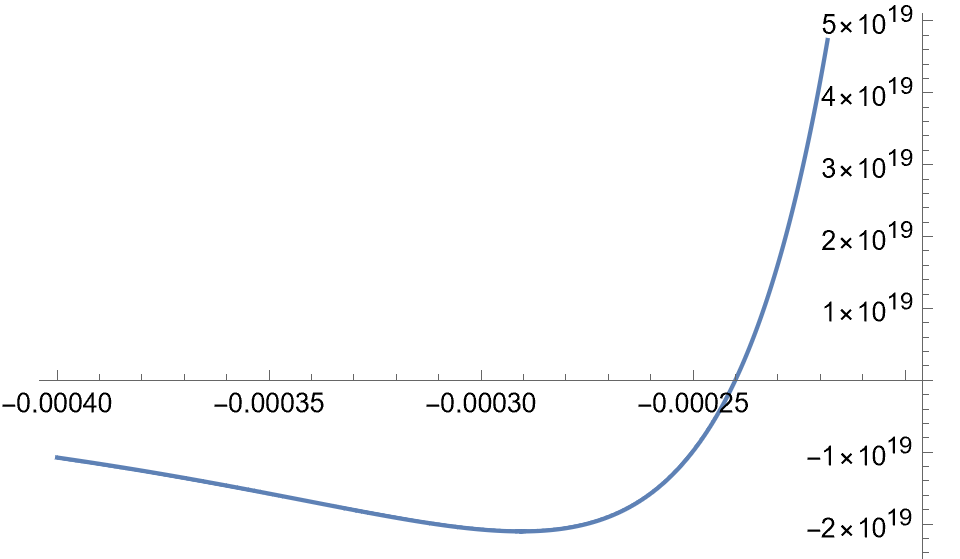
\includegraphics[width=0.4\textwidth]{fig/before_uplifting/before_uplifting.png}
  \end{center}

  \vspace{10pt}

  upliftした後のminimumは$10^{-15}$とでてきたので,確かによさそう.

\end{frame}

\subsection{カットしたスライド}

\begin{frame}[plain]
  \frametitle{\secname\thesubsection\ \subsecname}
  \label{cutted_10dSYM}
  

  \citeftwo{Arkani-Hamed_HigherDimensional_2002}{N. Arkani-Hamed, T. Gregoire, and J. Wacker}{Abe_SuperfieldDescription_2012}{H. Abe, T. Kobayashi, H. Ohki, and K. Sumita}

  \textcolor{DarkMagenta}{カット}
  \color{gray}

  10次元$\mathcal{N}=1$超対称ヤン=ミルズ理論の作用
  \begin{equation}
    S
    =
    \int\dd^{10}X\sqrt{-G}
    \frac{1}{g^2}\text{Tr}\ \left[
    -\frac{1}{4}F^{MN}F_{MN}+\frac{i}{2}\bar{\lambda}\Gamma^{M}D_{M}\lambda
    \right]
    \label{10dSYM}
  \end{equation}

  ただし,
  \begin{equation}
    g:\text{coupling constant}
    ,\
    G_{MN}:\text{10次元での計量\ $M,N=0,1,\cdots,9$}
    \nonumber
  \end{equation}
  であり,
  \begin{align}
    &
    F_{MN}
    =
    \partial_{M}A_{N}-\partial_{N}A_{M}
    -
    i[A_{M},A_{N}]
    \text{:field strengths}
    ,
    \nonumber
    \\
    &
    D_{M}\lambda
    =
    \partial_{M}\lambda
    -
    i[A_{M},\lambda]
    \text{:共変微分,これで局所ゲージ不変に}
    ,
    \nonumber
    \\
    &
    \lambda
    \text{:Majorana-Weyl\ $\rightarrow$\ 10次元で中性$+$カイラリティーが正}
    .
    \nonumber
  \end{align}
  それぞれゲージ群のアジョイント表現の足をもっていて,トレースはその行列の足についてとる.
\end{frame}


\begin{frame}[plain]
  \frametitle{\secname\thesubsection\ \subsecname}

  \citeftwo{Arkani-Hamed_HigherDimensional_2002}{N. Arkani-Hamed, T. Gregoire, and J. Wacker}{Abe_SuperfieldDescription_2012}{H. Abe, T. Kobayashi, H. Ohki, and K. Sumita}

  \textcolor{DarkMagenta}{カット}
  \color{gray}

  10次元のSYMの作用\eqref{10dSYM}は4次元$\mathcal{N}=1$の超場で表すと
  \begin{align}
    S
    &=
    \int\dd^{10}X
    \sqrt{-G}
    \left[
      \int\dd^{4}\theta\ \mathcal{K}
    \right.
    \nonumber
    \\
    &\hspace{2cm}
    \left.
      +
      \left\{
      \int\dd^{2}\theta\
      \left(
      \frac{1}{4g^2}\mathcal{W}^{\alpha}\mathcal{W}_{\alpha}
      +
      \mathcal{W}
      \right)
      +
      \text{h.c.}
      \right\}
    \right]
    .
    \label{10dactionsuperspace}
  \end{align}
  ただし,
  \begin{align}
    \mathcal{K}
    &=
    \frac{2}{g^2}h^{\bar{i}j}\text{Tr}
    \left[
    (\sqrt{2}\bar{\partial}_{\bar{i}}+\bar{\phi}_{\bar{i}})e^{-V}
    (\sqrt{2}\partial_{j}+\phi_{j})e^{V}
    \right.
    \nonumber
    \\
    &\hspace{6cm}
    \left.
      +
      \bar{\partial}_{\bar{i}}e^{-V}
      \partial_{i}e^{V}
    \right]
    ,
    \nonumber
    \\
    \mathcal{W}
     & =
    \frac{1}{g^2}\varepsilon^{\text{ijk}}
    e^{\ i}_{\text{i}}e^{\ j}_{\text{j}}e^{\ k}_{\text{k}}
    \text{Tr}\left[
      \sqrt{2}\phi_{i}
      \left(
      \partial_{j}\phi_{k}
      -
      \frac{1}{3\sqrt{2}}[\phi_{j},\phi_{k}]
      \right)
    \right]
    ,
    \nonumber
    \\
    \mathcal{W}_{\alpha}
    &=
    -
    \frac{1}{4}\overline{DD}e^{-V}D_{\alpha}e^{V}
    .
    \nonumber
  \end{align}

\end{frame}

\begin{frame}
  \frametitle{\thesection.\thesubsection\ \subsecname}

  \citefone{Abe_SuperfieldDescription_2012}{H. Abe, T. Kobayashi, H. Ohki, and K. Sumita}

  \color{DarkMagenta}
  (たぶん)私の研究のストーリーを語るのには関係ない.
  \color{gray}

  $\textcolor{Navy}{M^{(i)}}$がブロック対角化されているとする.つまり
  \begin{equation}
    \textcolor{Navy}{
      M^{(i)}
      =
      \begin{pmatrix}
        M_{N_{1}}^{(i)} &0 &\cdots & 0\\
        0&M_{N_{2}}^{(i)}&\cdots&0\\
        \vdots& \vdots& \ddots &\vdots \\
        0 & 0 & \cdots & M_{\tilde{N}}^{(i)}
      \end{pmatrix}
    }
    .
    \nonumber
  \end{equation}
  
  これは,ゲージが$U(N)\rightarrow U(N_1) \times\cdots\times U(\tilde{N})$に破れていることを意味する.

\end{frame}

\begin{frame}[plain]
  \frametitle{\secname\thesubsection\ \subsecname}
  \label{cutted_4dSUGRA}

  \citeftwo{Abe_SuperfieldDescription_2012}{H. Abe, T. Kobayashi, H. Ohki, and K. Sumita}{Kaku_SuperconformalUnified_1977}{M. Kaku, P. K. Townsend, and P. Van Nieuwenhuizen}

  \textcolor{DarkMagenta}{カット}
  \color{gray}

  作用
  \begin{align}
    S_{\mathcal{N}=1}
    &=
    \int\dd^4x\ \sqrt{-g^{C}}
    \left[\vphantom{\frac{1}{2}}\right.
    -3
    \int\dd^4\theta\ 
    \bar{C}Ce^{-K/3}
    \nonumber
    \\
    &\qquad
    +
    \left\{  
      \int\dd^2\theta\ 
      \left(  
        \frac{1}{4}\sum_{a=1}^{N}W^{a\alpha}W^{a}_{\alpha}+C^3W
      \right)
      +
      \text{h.c.}
    \right\}
    .
    \label{action_eff_SUGRA}
  \end{align}

  ただし
  \begin{itemize}
    \color{gray}
    \item 
    $C$はカイラル超場.
    \item 
    今回は,$C_{0}\equiv \left.C\right|_{\theta=\bar{\theta}=0}$は$e^{K_{0}/6}$にとる.
    \item 
    $W$はsuper potentialであり,カイラル超場$\Phi^{I}$の関数.
  \end{itemize}

\end{frame}

\begin{frame}[plain]
  \frametitle{\secname\thesubsection\ \subsecname}

  \citeftwo{Abe_SuperfieldDescription_2012}{H. Abe, T. Kobayashi, H. Ohki, and K. Sumita}{Kaku_SuperconformalUnified_1977}{M. Kaku, P. K. Townsend, and P. Van Nieuwenhuizen}

  \textcolor{DarkMagenta}{カット}
  \color{gray}

  ボゾンの寄与のみを拾ってくる.そのためには\eqref{action_eff_SUGRA}のうち
  \begin{equation}
    -3\int\dd^4\theta\ 
    \bar{C}Ce^{-K/3}
    +
    \left(  
      \int\dd^2\theta\ 
      C^3 W
      +
      \text{h.c.}
    \right)
    \nonumber
  \end{equation}
  のボゾンの寄与のみをみればよくて,計算すれば
  \begin{equation}
    V^{(F)}
    =
    -e^{K_{0}}
    (
      K^{I\bar{J}}D_{I}W_{0} D_{\bar{J}}\bar{W}_{0}
      -
      3|W|^2
    )
    .
    \nonumber
  \end{equation}

  記号はそれぞれ
  \begin{gather}
    K_{0}
    \equiv
    \left.K\right|_{\theta=\bar{\theta}=0}
    ,\ 
    W_{0}
    \equiv
    \left.W\right|_{\theta=\bar{\theta}=0}
    ,
    \nonumber
    \\
    D_{I}W_{0}
    \equiv
    (W_{I})_{0}
    +
    (K_{I})_{0}W_{0}
    ,\ 
    f_{I}
    \equiv
    \pdv{}{\Phi^{I}}f
    .
    \nonumber
  \end{gather}

\end{frame}

\subsection{なぜ\texorpdfstring{$M^{(i)}$}{Mi}を「磁場」というのか}

\begin{frame}[plain]
  \frametitle{\secname\thesubsection\ \subsecname}
  \label{why_flux}
  \color{DarkMagenta}

  第1トーラスの磁場は$F_{45}=\partial_{4}A_{5}-\partial_{5}A_{4}$なので,
  \begin{equation}
    \left\{
      \begin{alignedat}{1}
        z^{1}
        &\equiv
        \frac{1}{2}(y^4+\tau_{1}y^5)
        \nonumber
        \\
        \tilde{A}_{1}
        &\equiv
        -
        \frac{1}{\Im\tau_{1}}(\tau_{1}^{*}A_{4}-A_{5})
      \end{alignedat}
    \right.
  \end{equation}
  と
  \begin{equation}
    \ev*{A_{i}}
    =
    \frac{\pi}{\Im \tau_{i}}\textcolor{Navy}{M^{(i)}}\bar{z}_{i}
    \nonumber
  \end{equation}
  の条件に注意して計算すれば
  \begin{equation}
    F_{45}
    =
    \pi
    M^{1}
  \end{equation}
  となるから.他のトーラスも同様.もちろん一般にも計算できる.

\end{frame}

\setcounter{framenumber}{\value{Appendix}}
\end{document}
